\chapter{Implementacja}
W ramach pracy powstała minibiblioteka zawierająca moduły ułatwiające implementację protokołów działających w ramach WSN. Stanowi ona rozszerzenie biblioteki INET, zawierającej moduły dla standardu IEEE 802.15.4.

Biblioteka składa się z następujących modułów:
\begin{itemize}
	\item WSNNode --- złożony moduł ,,abstrakcyjny'' stanowiący bazę dla węzłów sieci. W jego skład wchodzą:
\paragraph{Moduł mobilności} Jest to moduł zarządzający położeniem oraz mobilnością węzła. Jako, że zakres pracy obejmuje węzły stacjonarne, jako wartość domyślna został przyjęty moduł StationaryMobility, który jedynie śledzi położenie węzła.
\paragraph{Źródło energii} Jako źródło energii wykorzystany został udostępniony przez Inet moduł prostego zasobnika energii (SimpleEnergyStorage).
\paragraph{Tablica interfejsów} Przechowuje informacje o interfejsach danego węzła. W przypadku objątych tą pracą symulacji jest to jeden interfejs radiowy.
\paragraph{Moduł stanu węzła} Jest to moduł informujący o aktualnym stanie węzła.
\paragraph{Moduł monitora} Jest to autorski moduł monitorujący poziom energii w węźle do celów statystycznych. Moduł w regularnych odstępach czasu emituje sygnał zawierający aktualną ilość energii w węźle.
\paragraph{Moduł warstwy sieciowej} Odpowiada za warstwę sieciową węzła. Zawierają się w nim moduły odpowiedzialne za trasowanie pakietów.
\paragraph{Moduł karty sieciowej} Jest to moduł symulujący kartę sieciową. Zawiera się w nim moduł odpowiadający za warstwę fizyczną oraz moduł łącza danych.
\begin{figure}[!htbp]
	\begin{center}
		\centering
		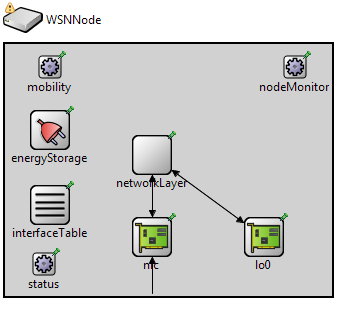
\includegraphics[scale=1]{\ImgPath/framework/node.png} 
	\end{center}
	\caption{Węzeł sieci}
	\label{abstractNode}
\end{figure}
\FloatBarrier
	\item WSNSensorNode - dziedziczy po WSNNode oraz zawiera dodatkowo moduł generujący pakiety
	\begin{figure}[!htbp]
	\begin{center}
		\centering
		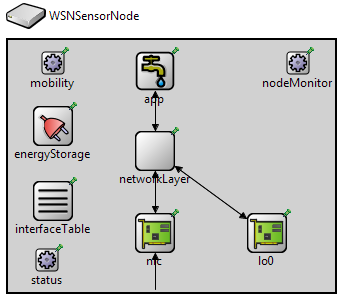
\includegraphics[scale=1]{\ImgPath/framework/sensor.png} 
	\end{center}
	\caption{Czujnik}
	\label{openlayers}
\end{figure}
\FloatBarrier
	\item WSNSinkNode - dziedziczy po WSNNode oraz zawiera dodatkowo moduł akcetujący pakiety od czujników
	\begin{figure}[!htbp]
	\begin{center}
		\centering
		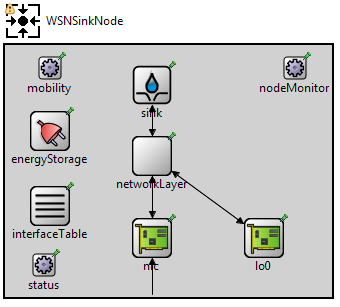
\includegraphics[scale=1]{\ImgPath/framework/sink.png} 
	\end{center}
	\caption{Stacja bazowa}
	\label{abstractNode}
\end{figure}
\FloatBarrier
	\item NodeCounter - moduł liczący działające węzły w sieci
	\item SimpleEnergyConsumer - moduł pobierający energię na żądanie
	\item VolatileStateBasedEnergyConsumer - moduł pobierający energię w zależności od ustawionego stanu z możliwością dynamicznej zmiany poboru mocy
\end{itemize}
\section{Protokoły}
Każda implementacja wybranego algorytmu trasowania wymaga stworzenia dwóch modułów. Jeden z nich dziedziczy po SimpleNetworkLayer, a drugi po NetworkProtocolBase.

Głównymi funkcjami, które jednocześnie wywoływane są przez silnik symulacji są handleSelfMessage, handleUpperPacket oraz handleLowerPacket.

\begin{minted}{cpp}
    virtual void handleSelfMessage(cMessage *msg) override;

    virtual void handleUpperPacket(cPacket *) override;

    virtual void handleLowerPacket(cPacket *) override;
\end{minted}
% flood jako akapit
\subsection{Flood}
W implementacji protokołu Flood wykorzystany został istniejący już moduł z biblioteki INET. Należało jedynie utworzyć  moduł będący warstwą sieciową, a następnie skonfigurować go, aby wykorzystywał moduł Flood z biblioteki INET.
\subsection{SPIN}
Protokół SPIN został zaimplementowany zgodnie z zaproponowanym w artykule \cite{Kulik2002} wariancie SPIN-RL.

Kod odpowiadający za logikę protokołu znajduje się w klasie SPIN, która dziedziczy po klasie NetworkProtocolBase oraz implementuje interfejs INetworkProtocol z biblioteki INET.

\begin{minted}{cpp}
class SPIN : public NetworkProtocolBase, public INetworkProtocol
\end{minted}

Moduł po otrzymaniu pakietu z wyższej warstwy dokonuje decyzji, czy węzeł ma dostatecznie dużo energii, aby przeprowadzić negocjację. W przypadku pozytywnej decyzji rozpoczynany jest proces negocjacji. W przeciwnym wypadku dane rozgłaszane są bezpośrednio, z pominięciem negocjacji. Obrazuje to poniższy fragment kodu.

\begin{minted}{cpp}
void SPIN::handleUpperPacket(cPacket *m)
{
    SPINDatagram *msg = encapsMsg(m, DATA);
    msg->setSeqNum(seqNum);
    seqNum++;

    if (isNegotiationViable()) {
        advertiseData(msg);
    } else {
        simpleSend(msg);
    }
    nbDataPacketsSent++;
}
\end{minted}

Teoretyczny opis protokołu SPIN nie zawiera algorytmu, który węzły powinny wykorzystywać przy podejmowaniu decyzji czy rozpoczęcie procesu negocjacji jest zasadne z punktu widzenia konserwacji zasobów energetycznych. W implementacji zaproponowany więc został algorytm wykorzystujący funkcję wygładzającą o poniższym wzorze ogólnym:
\[
	f(x) = \frac{k*x}{k - x + 1}
\]

Jako parametr k przyjęte zostało 1,2, a jako zmienną x stosunek aktualnej energii węzła do jego energii maksymalnej. Po podstawieniu otrzymuje się poniższy wzór, który został wykorzystany bezpośrednio w implementacji: 

\[
	f(E_{akt}, E_{max}) = \frac{1.2 * \frac{E_{akt}}{E_{max}}}{1.2 - \frac{E_{akt}}{E_{max}} + 1}
\]
Algorytm decyzyjny przedstawiony jest na poniższym listingu. Z przedziału [0, 1] losowana jest liczba, która następnie porównywana jest z wartością wcześniej opisanej funkcji. Jeżeli wylosowana liczba jest od niej mniejsza, podejmowana jest pozytywna decyzja o podjęciu negocjacji.
\begin{minted}{cpp}
bool SPIN::isNegotiationViable()
{
    double randomNumber = uniform(0, 1);
    double k = -1.2;
    double currentEnergyFrac = currentEnergy / maxEnergy;

    return randomNumber < (k*currentEnergyFrac / (k -
        currentEnergyFrac + 1));
}
\end{minted}
\subsection{LEACH}
Implementacja protokołu LEACH została wykonana na bazie implementacji z symulatora Castalia.
\subsection{ALEACH}
W ALEACH zmieniony został sposób wyboru lokalnego węzła bazowego. W implementacji wykorzystany został mechanizm dziedziczenia. Klasa ALEACH stanowi rozszerzenie wcześniej zaimplementowanej klasy LEACH. Jedyną zmianą jest przesłonięcie funkcji selectCH za pomocą tej zdefiniowanej na listingu poniżej, która realizuje założenia zawarte w akapicie \nameref{para:aleach} zawartym w sekcji \ref{subsec:leach}.
\begin{minted}{cpp}
void ALEACH::selectCH()
{
    ...
    double generalProb = (double)expectedCHNum / 
        (double)(numSensors - expectedCHNum * 
            (roundNumber % (numSensors / expectedCHNum) ));
    double currentEnergy = 
        energyStorage->getResidualCapacity().get();
    double currentStateProb = (currentEnergy / maxEnergy) *
        ((double) expectedCHNum / numSensors);
    ...
}
\end{minted}
\subsection{LEACH DCHS}
Protokół Leach DCHS zaimplementowany został w sposób analogiczny do protokołu ALEACH.
\begin{minted}{cpp}
void LEACH_DCHS::selectCH()
{
   ...
   probability = percentage / (1 - percentage * (roundNumber
       % (int)(1/percentage)))
       * (currentEnergy / maxEnergy +
       (notCHRounds / (1/percentage))
       * (1 - (currentEnergy / maxEnergy)));
   ...
}
\end{minted}
\section{Poprawa biblioteki INET}
Biblioteka INET jest aktywnie rozwijana oraz poprawiana. Jednakże część biblioteki implementująca moduły związane z sieciami czujnikowymi oraz sieciami typu BAN są zdecydowanie rzadziej aktualizowane. Konieczne okazało się więc stworzenie dedykowanych poprawek dla projektu.

\paragraph{Umożliwienie warstwie sieciowej dostępu do rssi} Problem został już wcześniej zasygnalizowany przez jednego z użytkowników, jednakże nie został on rozwiązany. Znajomość rssi jest niezbędna do prawidłowego działania algorytmów opartych na LEACH.

\paragraph{Dodanie możliwości zmiany modułu MAC w Ieee802154NarrowbandNic} W pierwotnej wersji rodzaj modułu MAC został zdefiniowany w sposób nie umożliwiający jego zmiany. Poprawka polega na wykorzystaniu zmiennej do przechowywania nazwy modułu MAC, który ma zostać dodany.

\paragraph{Poprawa modułu IPvXTrafGen, tak aby prawidłowo zachowywał się podczas deaktywacji węzła} Klasa implementująca moduł IPvXTrafGen dziedziczyła po klasie cSimpleModule, która nie wchodzi bezpośrednio w skład biblioteki INET (jest częścią \omnetpp). W związku z tym nie zostały w niej zaimplementowane funkcje związane z aktywnością węzła. Problem ten został naprawiony poprzez dokonanie zmiany rodzica klasy IPvXTrafGen na klasę ApplicationBase z biblioteki INET. Stanowi ona bazę dla klas implementujących zachowania modułów prostych należących do warstwy aplikacji. Udostępnione zostały również dzięki temu interfejsy związane z aktywacją oraz dezaktywacją węzła sieci.

\paragraph{Uzupełnienie modułu CSMA o funkcje obsługujące jego wyłączenie oraz ponowne włączenie} Przed poprawką, wyłącznie się symulowanego węzła (w wyniku zużycia energii) powodowało wystąpienie wyjątku i awaryjne zakończenie symulacji.

\paragraph{Obsługę przypadku, gdy pakiet dociera do wyłączonego już węzła} Dodana została obsługa przypadku brzegowego, w którym węzeł zostawał wyłączony podczas odbioru transmisji pakietu.
\begin{minted}{cpp}
bool Radio::handleNodeShutdown(...) {
    ...
    if (receptionTimer && receptionTimer->isScheduled())
        abortReception(receptionTimer);
    ...
}
\end{minted}